\section{Experiment \#2}\label{sec:experiment_two}

During Experiment \#1 in \cref{sec:experiment_one}, a few observations differed from our expectations. This was first of all regarding Linux having a lower energy consumption than Windows when comparing the clamp measurements, and second of all that the energy consumption of the idle test case is lower compared to the expected energy consumption of the different DUTs covered in \cref{subsec:expec_energy_consumption}. Because of this, a second experiment was introduced to look into this. One difference between the first and second experiments is how many test case measurements were made. In the first experiment, $120$ was made, but this was found in \cref{subsec:CockUse} to be too many. In this experiment, only $20$ measurements were made for all test cases except the idle case, where $55$ measurements were made.

\paragraph*{}
This experiment will aim to uncover why the idle test case had a lower energy consumption than expected. The expectation is that the low energy consumption measured on the idle test case also impacts the dynamic energy consumption on the different OSs, resulting in higher energy consumption for Windows.

\paragraph*{}
An example of the idle test case energy consumption being lower than expected can be observed in \cref{fig:TestCaseIdle_Cores_comparison_energy_without_outliers_PowerKomplett_avg_watts}. Here the idle test case's median energy consumption is reported by Intel Power Gadget to be $2.24W$ on the workstation, where the expectations were between $10W$ and $65W$. Because of this, some further investigation into the results was conducted. In terms of why the measurements were so low, a few things could have caused it, which will be covered now.


            \begin{figure}
                \centering
                \begin{tikzpicture}
                    \pgfplotsset{%
                        width=1\textwidth,
                        height=0.5\textheight
                    }
                    \begin{axis}[
                        xlabel={Start temperature},
                        ylabel={Average dynamic energy (watt)},
                    ]
                    
                    \end{axis}
                \end{tikzpicture} 
            \caption{A graph illustrating the energy consumption of Cores for test case TestCaseIdle with regards to the temperature of the DUT} \label{fig:TestCaseIdle_Cores}
            \end{figure}
            

\subsection{Implementation of Test Case Idle}

The implementation of idle test case was using \texttt{Thread.Sleep()} to represent a DUT doing nothing. An alternative way of representing a DUT doing nothing was to use \texttt{Task.Delay()}. The difference between these two implementations is that \texttt{Thread.Sleep()} will block the current thread\feetnote{https://learn.microsoft.com/en-us/dotnet/api/system.threading.thread.sleep?view=net-7.0}, and \texttt{Task.Delay()} will not block the current thread\feetnote{https://learn.microsoft.com/en-us/dotnet/api/system.threading.tasks.task.delay?view=net-7.0}. An experiment was conducted where the energy consumption was measured when \texttt{Task.Delay()} was used in stead, to see if the error was related to the implementation.

\paragraph*{Expectation:} The expectations in this experiment is to see no difference in the energy consumption between the two implementations of the idle case. This is expected as the DUT will not be doing anything, thus blocking/not blocking the thread is expected to have a limited impact.

\paragraph*{Results:} The results of this experiment showed that the measured energy consumption is similar when using \texttt{Thread.Sleep()} and \texttt{Task.Delay()}, as was expected. Because of this, the implementation will keep using \texttt{Thread.Sleep()} for the remainder of this work.

\subsection*{CPU-States}

Another possible cause of the issue of lower-than-expected measurements could be related to hardware. In the work by Fahad et al.\cite[]{fahad2019comparative} they experimented with disabling Core-states (C-states) on the CPU. These states include performance states (P-states) and C-states\cite[]{PCStat}, where the P-states provide a way to change the frequency and voltage of the CPU. Here P0 represents max performance and higher values of P underclocks the CPU. The C-states become relevant when the CPU is doing little to no work, where certain parts of the CPU will be turned off, resulting in reduced power consumption. 

\paragraph*{Expectation:} When considering the intuition, purpose and function of the different Power States, it shows that they can affect the power consumption of the DUT and could, depending on the circumstances, change the outcome of the experiments. This would cause the results of the experiments to be incorrect if the Power-States are not in the same state during all test cases. To get further information about the different states a CPU can be in, see \cref{app:CPU_states}

\paragraph*{Results:} To test whether the C-states were causing low energy consumption, they were disabled through the  BIOS. This was only possible on the workstation as the Surface devices had very limited options available. Running the experiments again with the C-states disable seemed to have little to no effect on the measurements. Looking more into the BIOS we discovered that the TUF B360M-PLUS GAMING motherboard had three modes, performance mode, Max power saving mode and automatic. Max power and performance mode would each change multiple BIOS settings where automatic would switch between performance and max power mode. The reason why just disabling the C-states did not impact the results, is expected to be a result of additional settings also needing to be changed. The specific changes made by max power and performance mode can be seen in \cref{tab:BIOSOptions}.

\begin{table}[]
    \centering
    \begin{tabular}{|l|l|l|l|}
    \hline
                                                                                   & \begin{tabular}[c]{@{}l@{}}Performance\\  Mode\end{tabular} & \begin{tabular}[c]{@{}l@{}}Max Power-\\ Saving Mode\end{tabular} & Default (Auto) \\ \hline
    Intell(R) SpeedStep                                                            & Disabled                                                    & Enabled                                                          & Auto           \\ \hline
    \begin{tabular}[c]{@{}l@{}}Long Duration \\ Package Power Limit\end{tabular}   & 4095                                                        & Auto                                                             & Auto           \\ \hline
    \begin{tabular}[c]{@{}l@{}}Package Power\\ Time Window\end{tabular}            & 127                                                         & Auto                                                             & Auto           \\ \hline
    Short Duration Power Limit                                                     & 4095                                                        & Auto                                                             & Auto           \\ \hline
    \begin{tabular}[c]{@{}l@{}}CPU Core/Cache\\ Current Limit\end{tabular}         & 255.50                                                      & Auto                                                             & Auto           \\ \hline
    \begin{tabular}[c]{@{}l@{}}PCI Express-\\ Native Power Management\end{tabular} & 255.50                                                      & Enabled                                                          & 255.50         \\ \hline
    Native ASPM                                                                    & Disabled                                                    & Enabled                                                          & Disabled       \\ \hline
    PCH DMI ASPM                                                                   & Disabled                                                    & L0sL1                                                            & Disabled       \\ \hline
    ASPM                                                                           & Disabled                                                    & L0sL1                                                            & Disabled       \\ \hline
    DMI Link ASPM Control                                                          & Disabled                                                    & L0sL1                                                            & Disabled       \\ \hline
    PEG - ASPM                                                                     & Disabled                                                    & ASPM L0sL1                                                       & Disabled       \\ \hline
    \begin{tabular}[c]{@{}l@{}}Intel(R) Speed-\\ Shift Technology\end{tabular}     & Disabled                                                    & Enabled                                                          & Enabled        \\ \hline
    CPU C-states                                                                   & Disabled                                                    & Enabled                                                          & Auto           \\ \hline
    Package C State Limit                                                          & CO/C1                                                       & C10                                                              & C10            \\ \hline
    RC6(Render Standby)                                                            & Disabled                                                    & Enabeld                                                          & Auto           \\ \hline
    Aggressive LPM support                                                         & Disabled                                                    & Enabled                                                          & Enabled        \\ \hline
    \end{tabular}
    \caption{These are the different BIOS setting that change based on which Performance mode is selected}
    \label{tab:BIOSOptions}
\end{table}

When performance mode is enabled, a comparison of the energy measurements from the different measuring instruments can be seen in \cref{fig:TestCaseIdle_Cores_comparison_energy_without_outliers_PowerKomplett_avg_watts_exp2}. For the workstation the limits for the energy consumption is set to be between $10$ and $65$ for the CPU and between $28.2$ and $113$ for the entire system, as presented in \cref{subsec:expec_energy_consumption}. Both values are relevant in this case as the software measurement instruments only measure the CPU while the clamp measure the entire system. According to \cref{fig:TestCaseIdle_Cores_comparison_energy_without_outliers_PowerKomplett_avg_watts_exp2}, all measuring instruments reports an energy consumption between these limits for Windows, where Intel Power Gadget is $25.9$, LHM is $23.57$ and the workstation is $107.74$. For Linux however, the measurements from the first and second experiments remain the same. This could indicate that Linux overwrites the C-states of the CPU, but this is a subject for future work.


            \begin{figure}
                \centering
                \begin{tikzpicture}
                    \pgfplotsset{%
                        width=1\textwidth,
                        height=0.5\textheight
                    }
                    \begin{axis}[
                        xlabel={Start temperature},
                        ylabel={Average dynamic energy (watt)},
                    ]
                    
                    \end{axis}
                \end{tikzpicture} 
            \caption{A graph illustrating the energy consumption of Cores for test case TestCaseIdle with regards to the temperature of the DUT} \label{fig:TestCaseIdle_Cores}
            \end{figure}
            

The results show an increased energy consumption for both hardware and software measuring instruments for Windows. This shows the power saving abilities of the C-states build into the motherboard and CPU. Given the different test cases, the only test case expected to enter another C-state than C0 is the idle test case. Because of this, it makes sense to disable the C-states. Some sources mention it might be possible to control the C-states through the OS\cite{CMete,CLinux}, but this was not prioritized and it is therefore a subject for future work. Given that it is only on the workstation that we can disable the C-States through the bios, a second experiment will be conducted with the C-states disabled for this DUT only.
